\documentclass{gescons}

\genre {Atualizações}
\author{Roberta Bouchardet}
\authorrole{Coordenadora da Escola de Editores}
\title{Nova Escola de Editores Impulsiona Formação Editoriológica na Editares}

\begin{document}
    \makeentrevistatitle
    %\maketitle

    %\fullwidthimage{fields}{b}

    %\coverart{back/editorial}
    \coverart{../fundo-generico.png}
    
    
\begin{center}
    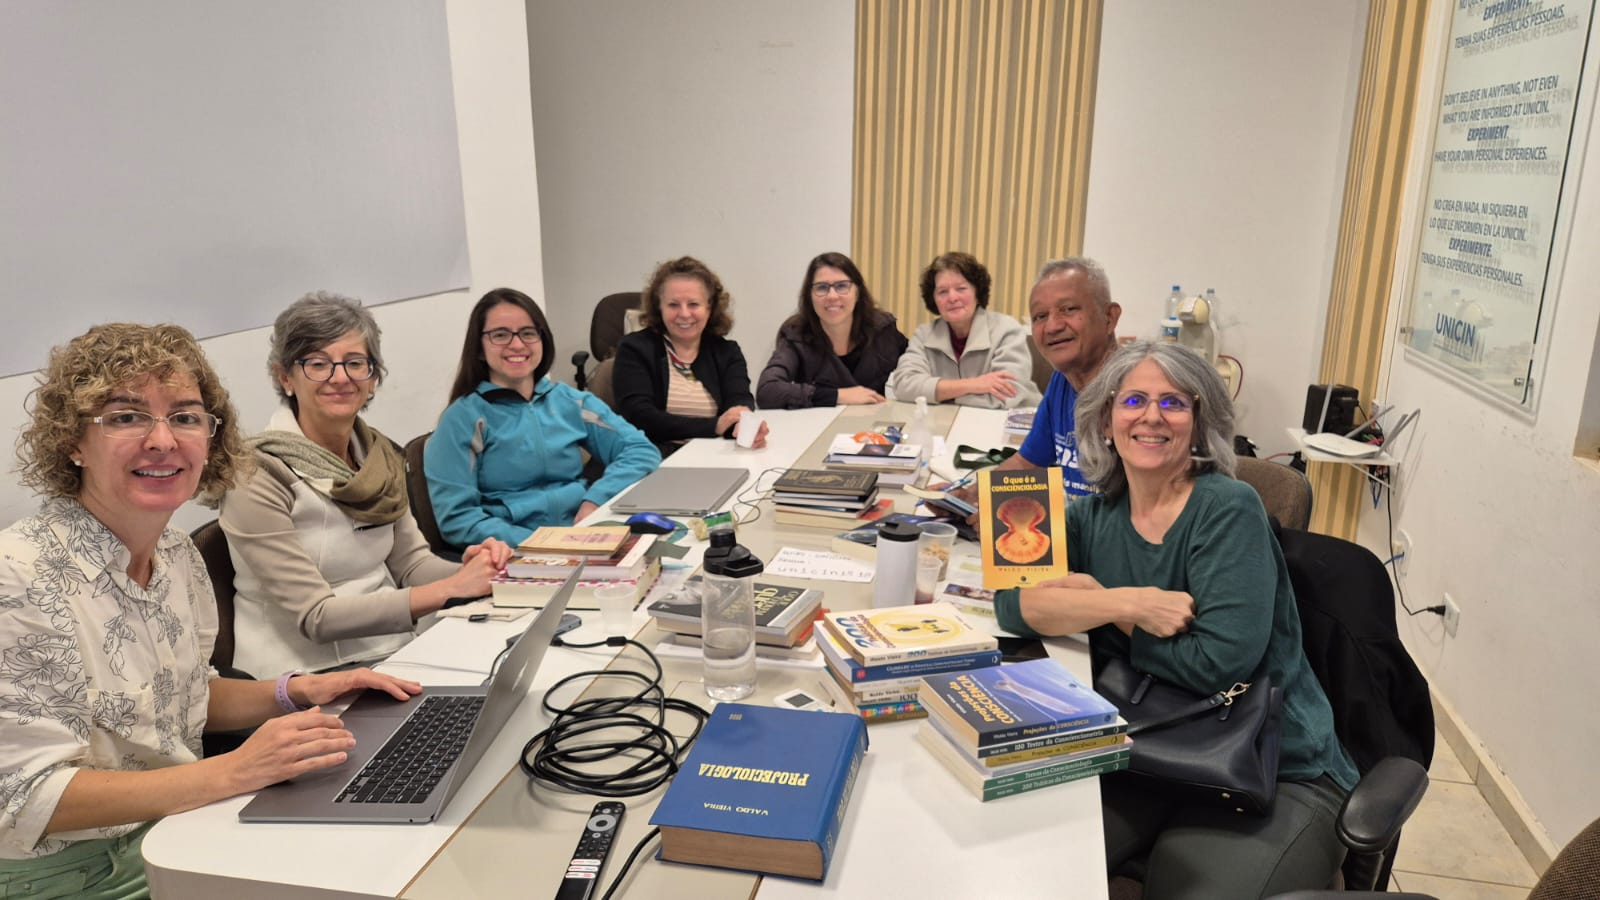
\includegraphics[height=10cm]{articles/atualizacoes/fotos/escola-editores/escola-editores4.jpeg} 
\end{center}
    
    \begin{multicols}{2}

%\section{Nova Escola de Editores impulsiona formação editoriológica na Editares}\label{nova-escola-de-editores-impulsiona-formauxe7uxe3o-editorioluxf3gica-na-editares}

Em julho de 2025, teve início a~\emph{Escola de Editores Conscienciológicos.} Trata-se de iniciativa inédita, objetivando formar e~qualificar voluntários do \emph{Conselho Editorial.} O~curso foi formulado pelos atuais conselheiros, ex-gestores da Editares, voluntários da UNICIN e~da CCCI com experiência no processo editorial. \textbf{A meta é~ampliar o~número de editores, qualificar as publicações, otimizar o~fluxo editorial e~ampliar a~interação entre os editores mais experientes com os novos.}

A \emph{Escola} responde à~crescente demanda de autores e~livros. A~proposta ganhou corpo com apoio da UNICIN, dentro do movimento de reestruturação institucional realizado em 2025. Com 11 módulos quinzenais aos domingos, em formato híbrido, o~curso terminou em dezembro deste ano, combinando teoria e~prática editorial.

A expectativa é~consolidar a~formação como etapa contínua da atuação editorial na CCCI, atraindo novos voluntários. A~turma piloto serviu de base para ajustesoara novas edições ou formatos gravados.

Estamos empolgados com as possibilidades que esse projeto pode gerar!


\begin{center}
    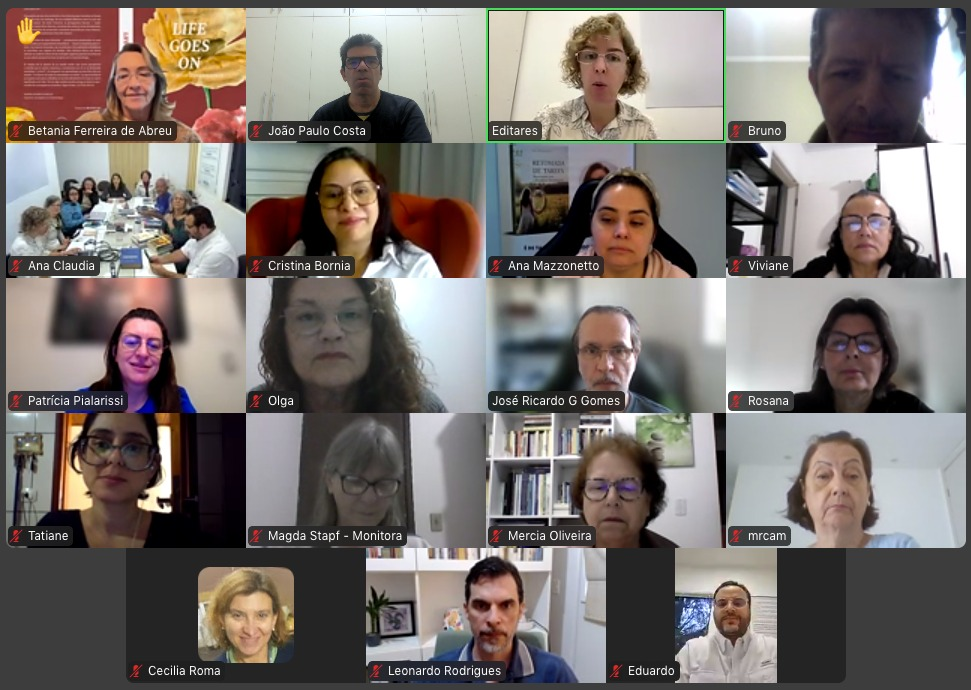
\includegraphics[width=9cm]{articles/atualizacoes/fotos/escola-editores/escola-editores1.jpeg} 
\end{center}


    \end{multicols}
\end{document}

